% vim: set spell spelllang=en tw=100 et sw=4 sts=4 foldmethod=marker foldmarker={{{,}}} :

\documentclass{beamer}

\usepackage{tikz}
\usepackage{xcolor}
\usepackage{complexity}
\usepackage{hyperref}
\usepackage{microtype}
\usepackage{amsmath}                   % \operatorname
\usepackage{amsfonts}                  % \mathcal
\usepackage{amssymb}                   % \nexists
\usepackage{gnuplot-lua-tikz}          % graphs
\usepackage[vlined]{algorithm2e} % algorithms

\usetikzlibrary{shapes, arrows, shadows, calc, positioning, fit}
\usetikzlibrary{decorations.pathreplacing, decorations.pathmorphing, shapes.misc}
\usetikzlibrary{tikzmark}

\newcommand*\circled[1]{\tikz[baseline=(char.base)]{
            \node[shape=circle,draw,inner sep=0pt] (char) {#1};}}

\definecolor{uofguniversityblue}{rgb}{0, 0.219608, 0.396078}

\definecolor{uofgheather}{rgb}{0.356863, 0.32549, 0.490196}
\definecolor{uofgaquamarine}{rgb}{0.603922, 0.72549, 0.678431}
\definecolor{uofgslate}{rgb}{0.309804, 0.34902, 0.380392}
\definecolor{uofgrose}{rgb}{0.823529, 0.470588, 0.709804}
\definecolor{uofgmocha}{rgb}{0.709804, 0.564706, 0.47451}

\definecolor{uofglawn}{rgb}{0.517647, 0.741176, 0}
\definecolor{uofgcobalt}{rgb}{0, 0.615686, 0.92549}
\definecolor{uofgturquoise}{rgb}{0, 0.709804, 0.819608}
\definecolor{uofgsunshine}{rgb}{1.0, 0.862745, 0.211765}
\definecolor{uofgpumpkin}{rgb}{1.0, 0.72549, 0.282353}
\definecolor{uofgthistle}{rgb}{0.584314, 0.070588, 0.447059}
\definecolor{uofgpillarbox}{rgb}{0.701961, 0.047059, 0}
\definecolor{uofglavendar}{rgb}{0.356863, 0.301961, 0.580392}

% {{{ theme things
\useoutertheme[footline=authortitle]{miniframes}
\useinnertheme{rectangles}

\setbeamerfont{block title}{size={}}
\setbeamercolor*{structure}{fg=uofguniversityblue}
\setbeamercolor*{palette primary}{use=structure,fg=black,bg=white}
\setbeamercolor*{palette secondary}{use=structure,fg=black,bg=uofgcobalt}
\setbeamercolor*{palette tertiary}{use=structure,fg=white,bg=uofguniversityblue}
\setbeamercolor*{palette quaternary}{fg=white,bg=black}

\setbeamercolor*{titlelike}{parent=palette primary}

\beamertemplatenavigationsymbolsempty

\setbeamertemplate{title page}
{
    \begin{tikzpicture}[remember picture, overlay]
        \node [anchor=center, fill=white, fill opacity=0.8, text opacity=1, inner sep=0.2cm, shift={(0cm,0.3cm)}] at (current page.center) {
            \begin{minipage}{\paperwidth}
                \centering
                {\usebeamerfont{title}\inserttitle}
                \vskip0.2cm
                {\usebeamerfont{author}\insertauthor \quad \insertinstitute}
            \end{minipage}
        };
    \end{tikzpicture}

    \begin{tikzpicture}[remember picture, overlay]
        \node at (current page.north west) {\begin{tikzpicture}[remember picture, overlay]\fill
        [fill=uofguniversityblue, anchor=north west] (0, 0) rectangle (\paperwidth, -1.5cm);\end{tikzpicture}};
        \node [anchor=north west, shift={(0.2cm,-0.2cm)}] at (current page.north west) {\includegraphics*[keepaspectratio=true,scale=0.5]{UoG_keyline.pdf}};
    \end{tikzpicture}
}

\setbeamertemplate{section page}
{
    \begin{centering}
        \begin{beamercolorbox}[sep=12pt,center]{part title}
            \usebeamerfont{section title}\insertsection\par
        end{beamercolorbox}
    \end{centering}
}

\newcommand{\frameofframes}{/}
\newcommand{\setframeofframes}[1]{\renewcommand{\frameofframes}{#1}}

\makeatletter
\setbeamertemplate{footline}
{%
    \begin{beamercolorbox}[colsep=1.5pt]{upper separation line foot}
    \end{beamercolorbox}
    \begin{beamercolorbox}[ht=2.5ex,dp=1.125ex,%
        leftskip=.3cm,rightskip=.3cm plus1fil]{author in head/foot}%
        \leavevmode{\usebeamerfont{author in head/foot}\insertshortauthor}%
        \hfill%
        {\usebeamerfont{institute in head/foot}\usebeamercolor[fg]{institute in head/foot}\insertshortinstitute}%
    \end{beamercolorbox}%
    \begin{beamercolorbox}[ht=2.5ex,dp=1.125ex,%
        leftskip=.3cm,rightskip=.3cm plus1fil]{title in head/foot}%
        {\usebeamerfont{title in head/foot}\insertshorttitle}%
        \hfill%
        {\usebeamerfont{frame number}\usebeamercolor[fg]{frame number}\insertframenumber~\frameofframes~\inserttotalframenumber}
    \end{beamercolorbox}%
    \begin{beamercolorbox}[colsep=1.5pt]{lower separation line foot}
    \end{beamercolorbox}
}

% }}}

\title{Parallel Search, Backjumping, and Brittle Skeletons}
\author{Ciaran McCreesh and Patrick Prosser}

\begin{document}

{
    \usebackgroundtemplate{
        \tikz[overlay, remember picture]
        \node[at=(current page.south), anchor=south, inner sep=0pt]{\includegraphics*[keepaspectratio=true, width=\paperwidth]{background.jpg}};
    }
    \begin{frame}[plain,noframenumbering]
        \titlepage
    \end{frame}
}

\begin{frame}{The Subgraph Isomorphism Problem}

    \centering
    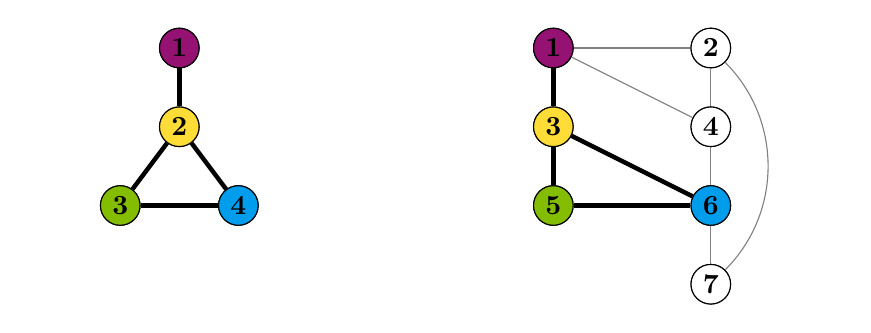
\begin{tikzpicture}%{{{
        \node at (-1, 0) { ~ };
        \node at (9, 0) { ~ };

        \node <1> [draw, circle, fill=white, inner sep=2pt, font=\bfseries] (Na) at (0.75,  0) {1};
        \node <1> [draw, circle, fill=white, inner sep=2pt, font=\bfseries] (Nb) at (0.75, -1) {2};
        \node <1> [draw, circle, fill=white, inner sep=2pt, font=\bfseries] (Nc) at (0, -2) {3};
        \node <1> [draw, circle, fill=white, inner sep=2pt, font=\bfseries] (Nd) at (1.5, -2) {4};

        \node <2> [draw, circle, fill=uofgthistle, inner sep=2pt, font=\bfseries] (Na) at (0.75,  0) {1};
        \node <2> [draw, circle, fill=uofgsunshine, inner sep=2pt, font=\bfseries] (Nb) at (0.75, -1) {2};
        \node <2> [draw, circle, fill=uofglawn, inner sep=2pt, font=\bfseries] (Nc) at (0, -2) {3};
        \node <2> [draw, circle, fill=uofgcobalt, inner sep=2pt, font=\bfseries] (Nd) at (1.5, -2) {4};

        \tikzstyle{edge} = [ultra thick];
        \tikzstyle{ledge} = [color = black!50!white];

        \draw <1> [ledge] (Na) -- (Nb);
        \draw <1> [ledge] (Nb) -- (Nc);
        \draw <1> [ledge] (Nc) -- (Nd);
        \draw <1> [ledge] (Nb) -- (Nd);

        \draw <2> [edge] (Na) -- (Nb);
        \draw <2> [edge] (Nb) -- (Nc);
        \draw <2> [edge] (Nc) -- (Nd);
        \draw <2> [edge] (Nb) -- (Nd);

        \node <1> [draw, circle, fill=white, inner sep=2pt, font=\bfseries] (N1) at (5.5,  0) {1};
        \node <1> [draw, circle, fill=white, inner sep=2pt, font=\bfseries] (N2) at (7.5,  0) {2};
        \node <1> [draw, circle, fill=white, inner sep=2pt, font=\bfseries] (N3) at (5.5, -1) {3};
        \node <1> [draw, circle, fill=white, inner sep=2pt, font=\bfseries] (N4) at (7.5, -1) {4};
        \node <1> [draw, circle, fill=white, inner sep=2pt, font=\bfseries] (N5) at (5.5, -2) {5};
        \node <1> [draw, circle, fill=white, inner sep=2pt, font=\bfseries] (N6) at (7.5, -2) {6};
        \node <1> [draw, circle, fill=white, inner sep=2pt, font=\bfseries] (N7) at (7.5, -3) {7};

        \node <2> [draw, circle, fill=uofgthistle, inner sep=2pt, font=\bfseries] (N1) at (5.5,  0) {1};
        \node <2> [draw, circle, fill=white, inner sep=2pt, font=\bfseries] (N2) at (7.5,  0) {2};
        \node <2> [draw, circle, fill=uofgsunshine, inner sep=2pt, font=\bfseries] (N3) at (5.5, -1) {3};
        \node <2> [draw, circle, fill=white, inner sep=2pt, font=\bfseries] (N4) at (7.5, -1) {4};
        \node <2> [draw, circle, fill=uofglawn, inner sep=2pt, font=\bfseries] (N5) at (5.5, -2) {5};
        \node <2> [draw, circle, fill=uofgcobalt, inner sep=2pt, font=\bfseries] (N6) at (7.5, -2) {6};
        \node <2> [draw, circle, fill=white, inner sep=2pt, font=\bfseries] (N7) at (7.5, -3) {7};

        \draw [ledge] (N1) -- (N2);
        \draw [ledge] (N1) -- (N4);
        \draw [ledge] (N2) -- (N4);
        \draw [ledge] (N4) -- (N6);
        \draw [ledge] (N2) to [in=45, out=315] (N7);
        \draw [ledge] (N6) -- (N7);

        \draw <1> [ledge] (N1) -- (N3);
        \draw <1> [ledge] (N3) -- (N5);
        \draw <1> [ledge] (N3) -- (N6);
        \draw <1> [ledge] (N5) -- (N6);
        \draw <2> [edge] (N1) -- (N3);
        \draw <2> [edge] (N3) -- (N5);
        \draw <2> [edge] (N3) -- (N6);
        \draw <2> [edge] (N5) -- (N6);

    \end{tikzpicture}%}}}
    \\~

\end{frame}

\begin{frame}{Filtering}

    \centering
    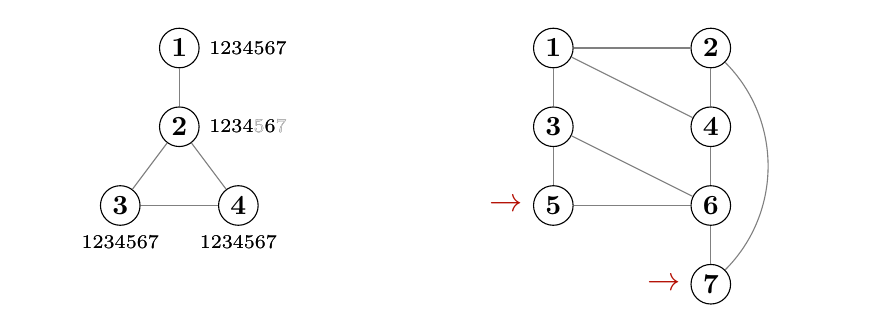
\begin{tikzpicture}%{{{
        \node at (-1, 0) { ~ };
        \node at (9, 0) { ~ };

        \node [draw, circle, fill=white, inner sep=2pt, font=\bfseries] (Na) at (0.75,  0) {1};
        \node [draw, circle, fill=white, inner sep=2pt, font=\bfseries] (Nb) at (0.75, -1) {2};
        \node [draw, circle, fill=white, inner sep=2pt, font=\bfseries] (Nc) at (0, -2) {3};
        \node [draw, circle, fill=white, inner sep=2pt, font=\bfseries] (Nd) at (1.5, -2) {4};

        \node <1-2> [right = 0 of Na, anchor = west, font=\scriptsize] { 1234567 };
        \node <1-2> [right = 0 of Nb, anchor = west, font=\scriptsize] { 1234567 };
        \node <1-2> [below = 0 of Nc, anchor = north, font=\scriptsize] { 1234567 };
        \node <1-2> [below = 0 of Nd, anchor = north, font=\scriptsize] { 1234567 };

        \node <3-4> [right = 0 of Na, anchor = west, font=\scriptsize] { 1234567 };
        \node <3-4> [right = 0 of Nb, anchor = west, font=\scriptsize] { 1234{\color{black!10!white}{5}}6{\color{black!10!white}{7}} };
        \node <3-4> [below = 0 of Nc, anchor = north, font=\scriptsize] { 1234567 };
        \node <3-4> [below = 0 of Nd, anchor = north, font=\scriptsize] { 1234567 };

        \tikzstyle{edge} = [ultra thick];
        \tikzstyle{ledge} = [color = black!50!white];

        \draw [ledge] (Na) -- (Nb);
        \draw [ledge] (Nb) -- (Nc);
        \draw [ledge] (Nc) -- (Nd);
        \draw [ledge] (Nb) -- (Nd);

        \node [draw, circle, fill=white, inner sep=2pt, font=\bfseries] (N1) at (5.5,  0) {1};
        \node [draw, circle, fill=white, inner sep=2pt, font=\bfseries] (N2) at (7.5,  0) {2};
        \node [draw, circle, fill=white, inner sep=2pt, font=\bfseries] (N3) at (5.5, -1) {3};
        \node [draw, circle, fill=white, inner sep=2pt, font=\bfseries] (N4) at (7.5, -1) {4};
        \node [draw, circle, fill=white, inner sep=2pt, font=\bfseries] (N5) at (5.5, -2) {5};
        \node [draw, circle, fill=white, inner sep=2pt, font=\bfseries] (N6) at (7.5, -2) {6};
        \node [draw, circle, fill=white, inner sep=2pt, font=\bfseries] (N7) at (7.5, -3) {7};

        \node <2-3> [left = 0 of N5, font=\large, text=uofgpillarbox] { $\rightarrow$ };
        \node <2-3> [left = 0 of N7, font=\large, text=uofgpillarbox] { $\rightarrow$ };

        \draw [ledge] (N1) -- (N2);
        \draw [ledge] (N1) -- (N4);
        \draw [ledge] (N2) -- (N4);
        \draw [ledge] (N4) -- (N6);
        \draw [ledge] (N2) to [in=45, out=315] (N7);
        \draw [ledge] (N6) -- (N7);

        \draw [ledge] (N1) -- (N3);
        \draw [ledge] (N3) -- (N5);
        \draw [ledge] (N3) -- (N6);
        \draw [ledge] (N5) -- (N6);

    \end{tikzpicture}%}}}
    \\~

\end{frame}

\begin{frame}{Backtracking Search}
    \centering
    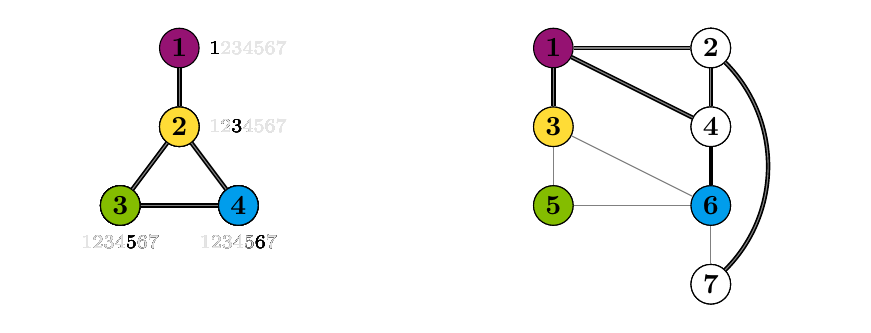
\begin{tikzpicture}%{{{
        \node at (-1, 0) { ~ };
        \node at (9, 0) { ~ };

        \node [draw, circle, fill=uofgthistle, inner sep=2pt, font=\bfseries] (Na) at (0.75,  0) {1};

        \node <1-5> [draw, circle, fill=white, inner sep=2pt, font=\bfseries] (Nb) at (0.75, -1) {2};
        \node <6-23> [draw, circle, fill=uofgsunshine, inner sep=2pt, font=\bfseries] (Nb) at (0.75, -1) {2};
        \node <24-> [draw, circle, fill=white, inner sep=2pt, font=\bfseries] (Nb) at (0.75, -1) {2};
        \node <26-> [draw, circle, fill=uofgsunshine, inner sep=2pt, font=\bfseries] (Nb) at (0.75, -1) {2};

        \node <1-10> [draw, circle, fill=white, inner sep=2pt, font=\bfseries] (Nc) at (0, -2) {3};
        \node <11-16> [draw, circle, fill=uofglawn, inner sep=2pt, font=\bfseries] (Nc) at (0, -2) {3};
        \node <17-18> [draw, circle, fill=white, inner sep=2pt, font=\bfseries] (Nc) at (0, -2) {3};
        \node <19-20> [draw, circle, fill=uofglawn, inner sep=2pt, font=\bfseries] (Nc) at (0, -2) {3};
        \node <21-22> [draw, circle, fill=white, inner sep=2pt, font=\bfseries] (Nc) at (0, -2) {3};
        \node <23> [draw, forbidden sign, fill=uofgpillarbox, inner sep=2pt, font=\bfseries] (Nc) at (0, -2) {3};
        \node <24-27> [draw, circle, fill=white, inner sep=2pt, font=\bfseries] (Nc) at (0, -2) {3};
        \node <28-> [draw, circle, fill=uofglawn, inner sep=2pt, font=\bfseries] (Nc) at (0, -2) {3};

        \node <1-15> [draw, circle, fill=white, inner sep=2pt, font=\bfseries] (Nd) at (1.5, -2) {4};
        \node <16> [draw, forbidden sign, fill=uofgpillarbox, inner sep=2pt, font=\bfseries] (Nd) at (1.5, -2) {4};
        \node <17-19> [draw, circle, fill=white, inner sep=2pt, font=\bfseries] (Nd) at (1.5, -2) {4};
        \node <20> [draw, forbidden sign, fill=uofgpillarbox, inner sep=2pt, font=\bfseries] (Nd) at (1.5, -2) {4};
        \node <21-23> [draw, circle, fill=white, inner sep=2pt, font=\bfseries] (Nd) at (1.5, -2) {4};
        \node <24-28> [draw, circle, fill=white, inner sep=2pt, font=\bfseries] (Nd) at (1.5, -2) {4};
        \node <29> [draw, circle, fill=uofgcobalt, inner sep=2pt, font=\bfseries] (Nd) at (1.5, -2) {4};

        \node <1> [right = 0 of Na, anchor = west, font=\scriptsize] { 1{\color{black!10!white}{234567}} };
        \node <1> [right = 0 of Nb, anchor = west, font=\scriptsize] { 1234{\color{black!10!white}{5}}6{\color{black!10!white}{7}} };
        \node <1> [below = 0 of Nc, anchor = north, font=\scriptsize] { 1234567 };
        \node <1> [below = 0 of Nd, anchor = north, font=\scriptsize] { 1234567 };

        \node <2-3> [right = 0 of Na, anchor = west, font=\scriptsize] { 1{\color{black!10!white}{234567}} };
        \node <2-3> [right = 0 of Nb, anchor = west, font=\scriptsize] { {\color{black!10!white}{1}}234{\color{black!10!white}{5}}6{\color{black!10!white}{7}} };
        \node <2-3> [below = 0 of Nc, anchor = north, font=\scriptsize] { {\color{black!10!white}{1}}234567 };
        \node <2-3> [below = 0 of Nd, anchor = north, font=\scriptsize] { {\color{black!10!white}{1}}234567 };

        \node <4-5> [right = 0 of Na, anchor = west, font=\scriptsize] { 1{\color{black!10!white}{234567}} };
        \node <4-5> [right = 0 of Nb, anchor = west, font=\scriptsize] { {\color{black!10!white}{1}}234{\color{black!10!white}{567}} };
        \node <4-5> [below = 0 of Nc, anchor = north, font=\scriptsize] { {\color{black!10!white}{1}}234567 };
        \node <4-5> [below = 0 of Nd, anchor = north, font=\scriptsize] { {\color{black!10!white}{1}}234567 };

        \node <6> [right = 0 of Na, anchor = west, font=\scriptsize] { 1{\color{black!10!white}{234567}} };
        \node <6> [right = 0 of Nb, anchor = west, font=\scriptsize] { {\color{black!10!white}{1}}2{\color{black!10!white}{34567}} };
        \node <6> [below = 0 of Nc, anchor = north, font=\scriptsize] { {\color{black!10!white}{1}}234567 };
        \node <6> [below = 0 of Nd, anchor = north, font=\scriptsize] { {\color{black!10!white}{1}}234567 };

        \node <7-8> [right = 0 of Na, anchor = west, font=\scriptsize] { 1{\color{black!10!white}{234567}} };
        \node <7-8> [right = 0 of Nb, anchor = west, font=\scriptsize] { {\color{black!10!white}{1}}2{\color{black!10!white}{34567}} };
        \node <7-8> [below = 0 of Nc, anchor = north, font=\scriptsize] { {\color{black!10!white}{12}}34567 };
        \node <7-8> [below = 0 of Nd, anchor = north, font=\scriptsize] { {\color{black!10!white}{12}}34567 };

        \node <9-10> [right = 0 of Na, anchor = west, font=\scriptsize] { 1{\color{black!10!white}{234567}} };
        \node <9-10> [right = 0 of Nb, anchor = west, font=\scriptsize] { {\color{black!10!white}{1}}2{\color{black!10!white}{34567}} };
        \node <9-10> [below = 0 of Nc, anchor = north, font=\scriptsize] { {\color{black!10!white}{123}}4{\color{black!10!white}{56}}7 };
        \node <9-10> [below = 0 of Nd, anchor = north, font=\scriptsize] { {\color{black!10!white}{123}}4{\color{black!10!white}{56}}7 };

        \node <11> [right = 0 of Na, anchor = west, font=\scriptsize] { 1{\color{black!10!white}{234567}} };
        \node <11> [right = 0 of Nb, anchor = west, font=\scriptsize] { {\color{black!10!white}{1}}2{\color{black!10!white}{34567}} };
        \node <11> [below = 0 of Nc, anchor = north, font=\scriptsize] { {\color{black!10!white}{123}}4{\color{black!10!white}{567}} };
        \node <11> [below = 0 of Nd, anchor = north, font=\scriptsize] { {\color{black!10!white}{123}}4{\color{black!10!white}{56}}7 };

        \node <12-13> [right = 0 of Na, anchor = west, font=\scriptsize] { 1{\color{black!10!white}{234567}} };
        \node <12-13> [right = 0 of Nb, anchor = west, font=\scriptsize] { {\color{black!10!white}{1}}2{\color{black!10!white}{34567}} };
        \node <12-13> [below = 0 of Nc, anchor = north, font=\scriptsize] { {\color{black!10!white}{123}}4{\color{black!10!white}{567}} };
        \node <12-13> [below = 0 of Nd, anchor = north, font=\scriptsize] { {\color{black!10!white}{123456}}7 };

        \node <14-16> [right = 0 of Na, anchor = west, font=\scriptsize] { 1{\color{black!10!white}{234567}} };
        \node <14-16> [right = 0 of Nb, anchor = west, font=\scriptsize] { {\color{black!10!white}{1}}2{\color{black!10!white}{34567}} };
        \node <14-16> [below = 0 of Nc, anchor = north, font=\scriptsize] { {\color{black!10!white}{123}}4{\color{black!10!white}{567}} };
        \node <14-16> [below = 0 of Nd, anchor = north, font=\scriptsize] { {\color{black!10!white}{1234567}} };

        \node <17> [right = 0 of Na, anchor = west, font=\scriptsize] { 1{\color{black!10!white}{234567}} };
        \node <17> [right = 0 of Nb, anchor = west, font=\scriptsize] { {\color{black!10!white}{1}}2{\color{black!10!white}{34567}} };
        \node <17> [below = 0 of Nc, anchor = north, font=\scriptsize] { {\color{black!10!white}{123}}4{\color{black!10!white}{56}}7 };
        \node <17> [below = 0 of Nd, anchor = north, font=\scriptsize] { {\color{black!10!white}{123}}4{\color{black!10!white}{56}}7 };

        \node <18-19> [right = 0 of Na, anchor = west, font=\scriptsize] { 1{\color{black!10!white}{234567}} };
        \node <18-19> [right = 0 of Nb, anchor = west, font=\scriptsize] { {\color{black!10!white}{1}}2{\color{black!10!white}{34567}} };
        \node <18-19> [below = 0 of Nc, anchor = north, font=\scriptsize] { {\color{black!10!white}{123456}}7 };
        \node <18-19> [below = 0 of Nd, anchor = north, font=\scriptsize] { {\color{black!10!white}{123}}4{\color{black!10!white}{56}}7 };

        \node <20> [right = 0 of Na, anchor = west, font=\scriptsize] { 1{\color{black!10!white}{234567}} };
        \node <20> [right = 0 of Nb, anchor = west, font=\scriptsize] { {\color{black!10!white}{1}}2{\color{black!10!white}{34567}} };
        \node <20> [below = 0 of Nc, anchor = north, font=\scriptsize] { {\color{black!10!white}{123456}}7 };
        \node <20> [below = 0 of Nd, anchor = north, font=\scriptsize] { {\color{black!10!white}{1234567}} };

        \node <21> [right = 0 of Na, anchor = west, font=\scriptsize] { 1{\color{black!10!white}{234567}} };
        \node <21> [right = 0 of Nb, anchor = west, font=\scriptsize] { {\color{black!10!white}{1}}2{\color{black!10!white}{34567}} };
        \node <21> [below = 0 of Nc, anchor = north, font=\scriptsize] { {\color{black!10!white}{123456}}7 };
        \node <21> [below = 0 of Nd, anchor = north, font=\scriptsize] { {\color{black!10!white}{123}}4{\color{black!10!white}{56}}7 };

        \node <22-23> [right = 0 of Na, anchor = west, font=\scriptsize] { 1{\color{black!10!white}{234567}} };
        \node <22-23> [right = 0 of Nb, anchor = west, font=\scriptsize] { {\color{black!10!white}{1}}2{\color{black!10!white}{34567}} };
        \node <22-23> [below = 0 of Nc, anchor = north, font=\scriptsize] { {\color{black!10!white}{1234567}} };
        \node <22-23> [below = 0 of Nd, anchor = north, font=\scriptsize] { {\color{black!10!white}{123}}4{\color{black!10!white}{56}}7 };

        \node <24> [right = 0 of Na, anchor = west, font=\scriptsize] { 1{\color{black!10!white}{234567}} };
        \node <24> [right = 0 of Nb, anchor = west, font=\scriptsize] { {\color{black!10!white}{1}}234{\color{black!10!white}{567}} };
        \node <24> [below = 0 of Nc, anchor = north, font=\scriptsize] { {\color{black!10!white}{1}}234567 };
        \node <24> [below = 0 of Nd, anchor = north, font=\scriptsize] { {\color{black!10!white}{1}}234567 };

        \node <25> [right = 0 of Na, anchor = west, font=\scriptsize] { 1{\color{black!10!white}{234567}} };
        \node <25> [right = 0 of Nb, anchor = west, font=\scriptsize] { {\color{black!10!white}{12}}34{\color{black!10!white}{567}} };
        \node <25> [below = 0 of Nc, anchor = north, font=\scriptsize] { {\color{black!10!white}{1}}234567 };
        \node <25> [below = 0 of Nd, anchor = north, font=\scriptsize] { {\color{black!10!white}{1}}234567 };

        \node <26> [right = 0 of Na, anchor = west, font=\scriptsize] { 1{\color{black!10!white}{234567}} };
        \node <26> [right = 0 of Nb, anchor = west, font=\scriptsize] { {\color{black!10!white}{12}}3{\color{black!10!white}{4567}} };
        \node <26> [below = 0 of Nc, anchor = north, font=\scriptsize] { {\color{black!10!white}{1}}234567 };
        \node <26> [below = 0 of Nd, anchor = north, font=\scriptsize] { {\color{black!10!white}{1}}234567 };

        \node <27> [right = 0 of Na, anchor = west, font=\scriptsize] { 1{\color{black!10!white}{234567}} };
        \node <27> [right = 0 of Nb, anchor = west, font=\scriptsize] { {\color{black!10!white}{12}}3{\color{black!10!white}{4567}} };
        \node <27> [below = 0 of Nc, anchor = north, font=\scriptsize] { {\color{black!10!white}{1234}}56{\color{black!10!white}{7}} };
        \node <27> [below = 0 of Nd, anchor = north, font=\scriptsize] { {\color{black!10!white}{1234}}56{\color{black!10!white}{7}} };

        \node <28> [right = 0 of Na, anchor = west, font=\scriptsize] { 1{\color{black!10!white}{234567}} };
        \node <28> [right = 0 of Nb, anchor = west, font=\scriptsize] { {\color{black!10!white}{12}}3{\color{black!10!white}{4567}} };
        \node <28> [below = 0 of Nc, anchor = north, font=\scriptsize] { {\color{black!10!white}{1234}}5{\color{black!10!white}{67}} };
        \node <28> [below = 0 of Nd, anchor = north, font=\scriptsize] { {\color{black!10!white}{1234}}56{\color{black!10!white}{7}} };

        \node <29> [right = 0 of Na, anchor = west, font=\scriptsize] { 1{\color{black!10!white}{234567}} };
        \node <29> [right = 0 of Nb, anchor = west, font=\scriptsize] { {\color{black!10!white}{12}}3{\color{black!10!white}{4567}} };
        \node <29> [below = 0 of Nc, anchor = north, font=\scriptsize] { {\color{black!10!white}{1234}}5{\color{black!10!white}{67}} };
        \node <29> [below = 0 of Nd, anchor = north, font=\scriptsize] { {\color{black!10!white}{12345}}6{\color{black!10!white}{7}} };

        \tikzstyle{edge} = [ultra thick];
        \tikzstyle{ledge} = [color = black!50!white];

        \draw <1-2> [ledge] (Na) -- (Nb);
        \draw <3-4> [edge] (Na) -- (Nb);
        \draw <5-> [ledge] (Na) -- (Nb);

        \draw <1-7> [ledge] (Nb) -- (Nc);
        \draw <1-7> [ledge] (Nb) -- (Nd);
        \draw <8-9> [edge] (Nb) -- (Nc);
        \draw <8-9> [edge] (Nb) -- (Nd);
        \draw <10-> [ledge] (Nb) -- (Nc);
        \draw <10-> [ledge] (Nb) -- (Nd);
        \draw <1-12> [ledge] (Nc) -- (Nd);
        \draw <13-14> [edge] (Nc) -- (Nd);
        \draw <15-> [ledge] (Nc) -- (Nd);

        \node [draw, circle, fill=uofgthistle, inner sep=2pt, font=\bfseries] (N1) at (5.5,  0) {1};

        \node <1-5> [draw, circle, fill=white, inner sep=2pt, font=\bfseries] (N2) at (7.5,  0) {2};
        \node <6-23> [draw, circle, fill=uofgsunshine, inner sep=2pt, font=\bfseries] (N2) at (7.5,  0) {2};
        \node <24-> [draw, circle, fill=white, inner sep=2pt, font=\bfseries] (N2) at (7.5,  0) {2};

        \node <1-25> [draw, circle, fill=white, inner sep=2pt, font=\bfseries] (N3) at (5.5, -1) {3};
        \node <26-> [draw, circle, fill=uofgsunshine, inner sep=2pt, font=\bfseries] (N3) at (5.5, -1) {3};

        \node <1-10> [draw, circle, fill=white, inner sep=2pt, font=\bfseries] (N4) at (7.5, -1) {4};
        \node <11-16> [draw, circle, fill=uofglawn, inner sep=2pt, font=\bfseries] (N4) at (7.5, -1) {4};
        \node <17-> [draw, circle, fill=white, inner sep=2pt, font=\bfseries] (N4) at (7.5, -1) {4};

        \node <1-27> [draw, circle, fill=white, inner sep=2pt, font=\bfseries] (N5) at (5.5, -2) {5};
        \node <28-> [draw, circle, fill=uofglawn, inner sep=2pt, font=\bfseries] (N5) at (5.5, -2) {5};

        \node <1-28> [draw, circle, fill=white, inner sep=2pt, font=\bfseries] (N6) at (7.5, -2) {6};
        \node <29-> [draw, circle, fill=uofgcobalt, inner sep=2pt, font=\bfseries] (N6) at (7.5, -2) {6};

        \node <1-18> [draw, circle, fill=white, inner sep=2pt, font=\bfseries] (N7) at (7.5, -3) {7};
        \node <19-20> [draw, circle, fill=uofglawn, inner sep=2pt, font=\bfseries] (N7) at (7.5, -3) {7};
        \node <21-> [draw, circle, fill=white, inner sep=2pt, font=\bfseries] (N7) at (7.5, -3) {7};

        \draw [ledge] (N6) -- (N7);
        \draw [ledge] (N3) -- (N5);
        \draw [ledge] (N3) -- (N6);
        \draw [ledge] (N5) -- (N6);

        \draw <1-2> [ledge] (N1) -- (N2);
        \draw <1-2> [ledge] (N1) -- (N4);
        \draw <1-2> [ledge] (N1) -- (N3);
        \draw <3-4> [edge] (N1) -- (N2);
        \draw <3-4> [edge] (N1) -- (N4);
        \draw <3-4> [edge] (N1) -- (N3);
        \draw <5-> [ledge] (N1) -- (N2);
        \draw <5-> [ledge] (N1) -- (N4);
        \draw <5-> [ledge] (N1) -- (N3);

        \draw <1-7> [ledge] (N2) -- (N4);
        \draw <1-7> [ledge] (N2) to [in=45, out=315] (N7);
        \draw <8-9> [edge] (N2) -- (N4);
        \draw <8-9> [edge] (N2) to [in=45, out=315] (N7);
        \draw <10-> [ledge] (N2) -- (N4);
        \draw <10-> [ledge] (N2) to [in=45, out=315] (N7);

        \draw <1-12> [ledge] (N4) -- (N6);
        \draw <15-> [ledge] (N4) -- (N6);
        \draw <13-14> [edge] (N4) -- (N6);

    \end{tikzpicture}%}}}
    \\~

\end{frame}

\begin{frame}{A Backtracking Algorithm}
    \small
    \begin{algorithm}[H]
    \DontPrintSemicolon
    \SetKwSwitch{Switch}{Case}{Other}{case}{of}{}{otherwise}{endcase}{endsw}
    \nl $\FuncSty{search}$ (Domains $D$) $\rightarrow$ Fail \KwSty{or} Success \;
    \nl \Begin{
        \nl \lIf {$D = \emptyset$}{$\KwSty{return}~\textnormal{Success}$}
        \nl $D_v \gets \textnormal{a domain in $D$ with minimum size}$ \;
        \nl \ForEach {$v' \in D_v~\textnormal{ordered by a heuristic}$}{
            \nl $D' \gets \FuncSty{clone}(D)$ \;
            \nl \Switch{$\FuncSty{assign}(D', v, v')$}{
                \nl \lCase{\textnormal{Fail~\KwSty{then}}}{keep going}
                \nl \Case{\textnormal{Success~\KwSty{then}}}{
                    \nl \Switch{$\FuncSty{search}(D' - D_v)$}{
                        \nl \lCase{\textnormal{Fail~\KwSty{then}}}{keep going}
                        \nl \lCase{\textnormal{Success~\KwSty{then}}}{$\KwSty{return}~\textnormal{Success}$}
                    }
                }
            }
        }
        \nl $\KwSty{return}~\textnormal{Fail}$ \;
    }
    \end{algorithm}
\end{frame}

\begin{frame}{Search as a Tree}
    \centering
    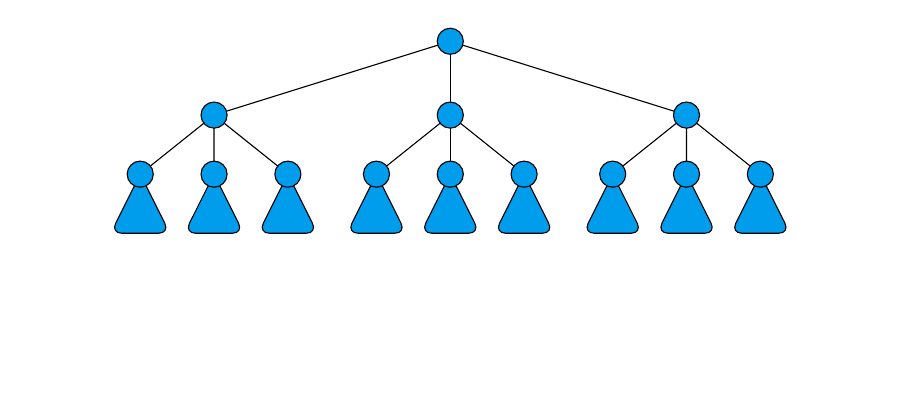
\begin{tikzpicture}[scale=0.75]%{{{
        \coordinate (R);

        \coordinate (N) at (R);

        \coordinate (N1) at ($(N) + (-4, -1.25)$);
        \coordinate (N2) at ($(N) + ( 0, -1.25)$);
        \coordinate (N3) at ($(N) + ( 4, -1.25)$);

        \foreach \na in {1, ..., 3}{
            \coordinate (N\na 1) at ($(N\na) + (-1.25, -1)$);
            \coordinate (N\na 2) at ($(N\na) + ( 0,    -1)$);
            \coordinate (N\na 3) at ($(N\na) + ( 1.25, -1)$);

            \foreach \nb in {1, ..., 3}{
                \coordinate (N\na\nb t1) at ($(N\na\nb) + (-0.5, -1)$);
                \coordinate (N\na\nb t2) at ($(N\na\nb) + ( 0.5, -1)$);

                \coordinate (N\na\nb s1) at ($(N\na\nb) + (-0.3, -0.6)$);
                \coordinate (N\na\nb s2) at ($(N\na\nb) + ( 0.3, -0.6)$);

                \coordinate (N\na\nb h1) at ($(N\na\nb) + (-1.5, -3)$);
                \coordinate (N\na\nb h2) at ($(N\na\nb) + ( 1.5, -3)$);
            }
        }

        \foreach \na in {1, ..., 3}{
            \draw (N) -- (N\na);
            \foreach \nb in {1, ..., 3}{
                \draw (N\na) -- (N\na\nb);
            }
        }

        \tikzstyle{t} = [draw, fill, fill=uofgcobalt, rounded corners];
        \foreach \na in {1, ..., 3}{
            \foreach \nb in {1, ..., 3}{
                \draw [t] (N\na\nb) -- (N\na\nb t1) -- (N\na\nb t2) -- cycle;
            }
        }

        \tikzstyle{c} = [draw, circle, fill, fill=uofgcobalt];
        \node [c] at (N) { };

        \foreach \na in {1, ..., 3}{
            \node [c] at (N\na) { };

            \foreach \nb in {1, ..., 3}{
                \node [c] at (N\na\nb) { };
            }
        }

        \node at (-7, -5.5) { }; \node at (7, -5.5) { };
    \end{tikzpicture}%}}}
    \\~
\end{frame}

\begin{frame}{Parallel Search}
    \centering
    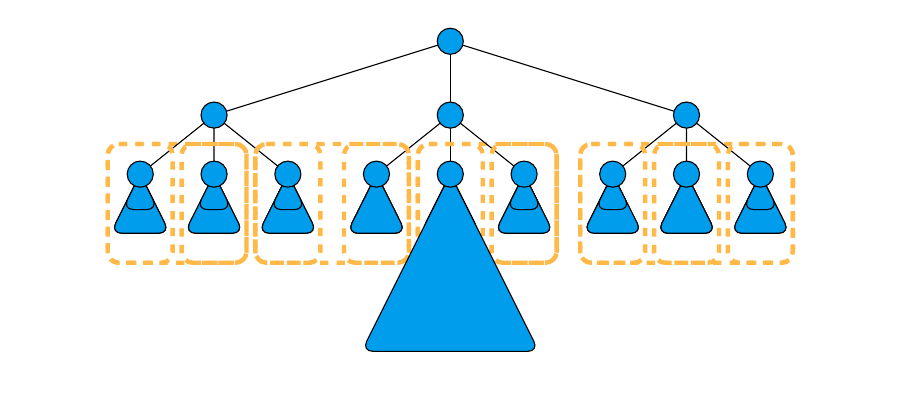
\begin{tikzpicture}[scale=0.75]%{{{
        \coordinate (R);

        \coordinate (N) at (R);

        \coordinate (N1) at ($(N) + (-4, -1.25)$);
        \coordinate (N2) at ($(N) + ( 0, -1.25)$);
        \coordinate (N3) at ($(N) + ( 4, -1.25)$);

        \foreach \na in {1, ..., 3}{
            \coordinate (N\na 1) at ($(N\na) + (-1.25, -1)$);
            \coordinate (N\na 2) at ($(N\na) + ( 0,    -1)$);
            \coordinate (N\na 3) at ($(N\na) + ( 1.25, -1)$);

            \foreach \nb in {1, ..., 3}{
                \coordinate (N\na\nb t1) at ($(N\na\nb) + (-0.5, -1)$);
                \coordinate (N\na\nb t2) at ($(N\na\nb) + ( 0.5, -1)$);

                \coordinate (N\na\nb s1) at ($(N\na\nb) + (-0.3, -0.6)$);
                \coordinate (N\na\nb s2) at ($(N\na\nb) + ( 0.3, -0.6)$);

                \coordinate (N\na\nb h1) at ($(N\na\nb) + (-1.5, -3)$);
                \coordinate (N\na\nb h2) at ($(N\na\nb) + ( 1.5, -3)$);
            }
        }

        \tikzstyle{p} = [draw, rounded corners, dashed, color=uofgpumpkin, ultra thick];
        \draw <1-2> [p] ($(N11) + (-0.55, 0.51)$) -- ($(N12) + (0.55, 0.51)$) -- ($(N12) + (0.55, -1.5)$) -- ($(N11) + (-0.55, -1.5)$) -- cycle;
        \draw <1-2> [p] ($(N13) + (-0.55, 0.51)$) -- ($(N21) + (0.55, 0.51)$) -- ($(N21) + (0.55, -1.5)$) -- ($(N13) + (-0.55, -1.5)$) -- cycle;
        \draw <1-2> [p] ($(N22) + (-0.55, 0.51)$) -- ($(N23) + (0.55, 0.51)$) -- ($(N23) + (0.55, -1.5)$) -- ($(N22) + (-0.55, -1.5)$) -- cycle;
        \draw <1-2> [p] ($(N31) + (-0.55, 0.51)$) -- ($(N33) + (0.55, 0.51)$) -- ($(N33) + (0.55, -1.5)$) -- ($(N31) + (-0.55, -1.5)$) -- cycle;

        \foreach \na in {1, ..., 3}{
            \draw (N) -- (N\na);
            \foreach \nb in {1, ..., 3}{
                \draw (N\na) -- (N\na\nb);
            }
        }

        \tikzstyle{t} = [draw, fill, fill=uofgcobalt, rounded corners];
        \foreach \na in {1, ..., 3}{
            \foreach \nb in {1, ..., 3}{
                \draw <1> [t] (N\na\nb) -- (N\na\nb t1) -- (N\na\nb t2) -- cycle;
                \draw <3> [t] (N\na\nb) -- (N\na\nb t1) -- (N\na\nb t2) -- cycle;
            }
        }

        \foreach \na in {1, ..., 3}{
            \foreach \nb in {1, ..., 3}{
                \draw <3> [p] ($(N\na\nb) + (-0.55, 0.51)$) -- ($(N\na\nb) + (0.55, 0.51)$) --
                ($(N\na\nb) + (0.55, -1.5)$) -- ($(N\na\nb) + (-0.55, -1.5)$) -- cycle;
            }
        }

        \draw <2> [t] (N11) -- (N11s1) -- (N11s2) -- cycle;
        \draw <2> [t] (N12) -- (N12s1) -- (N12s2) -- cycle;
        \draw <2> [t] (N13) -- (N13s1) -- (N13s2) -- cycle;

        \draw <2> [t] (N21) -- (N21t1) -- (N21t2) -- cycle;
        \draw <2> [t] (N22) -- (N22h1) -- (N22h2) -- cycle;
        \draw <2> [t] (N23) -- (N23s1) -- (N23s2) -- cycle;

        \draw <2> [t] (N31) -- (N31s1) -- (N31s2) -- cycle;
        \draw <2> [t] (N32) -- (N32t1) -- (N32t2) -- cycle;
        \draw <2> [t] (N33) -- (N33s1) -- (N33s2) -- cycle;

        \tikzstyle{c} = [draw, circle, fill, fill=uofgcobalt];
        \node [c] at (N) { };

        \foreach \na in {1, ..., 3}{
            \node [c] at (N\na) { };

            \foreach \nb in {1, ..., 3}{
                \node [c] at (N\na\nb) { };
            }
        }

        \node at (-7, -5.5) { }; \node at (7, -5.5) { };
    \end{tikzpicture}%}}}
    \\~
\end{frame}

\begin{frame}{Work-Stealing is Not Just About Balance}
    \centering
    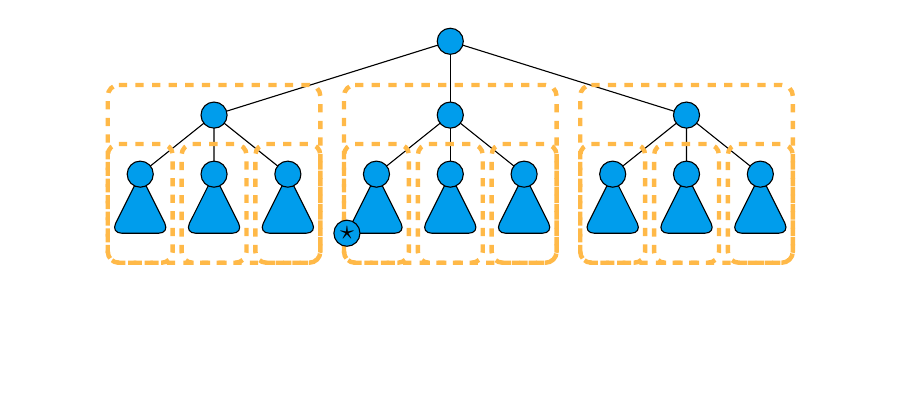
\begin{tikzpicture}[scale=0.75]%{{{
        \coordinate (R);

        \coordinate (N) at (R);

        \coordinate (N1) at ($(N) + (-4, -1.25)$);
        \coordinate (N2) at ($(N) + ( 0, -1.25)$);
        \coordinate (N3) at ($(N) + ( 4, -1.25)$);

        \foreach \na in {1, ..., 3}{
            \coordinate (N\na 1) at ($(N\na) + (-1.25, -1)$);
            \coordinate (N\na 2) at ($(N\na) + ( 0,    -1)$);
            \coordinate (N\na 3) at ($(N\na) + ( 1.25, -1)$);

            \foreach \nb in {1, ..., 3}{
                \coordinate (N\na\nb t1) at ($(N\na\nb) + (-0.5, -1)$);
                \coordinate (N\na\nb t2) at ($(N\na\nb) + ( 0.5, -1)$);

                \coordinate (N\na\nb s1) at ($(N\na\nb) + (-0.3, -0.6)$);
                \coordinate (N\na\nb s2) at ($(N\na\nb) + ( 0.3, -0.6)$);

                \coordinate (N\na\nb h1) at ($(N\na\nb) + (-1.5, -3)$);
                \coordinate (N\na\nb h2) at ($(N\na\nb) + ( 1.5, -3)$);
            }
        }

        \tikzstyle{p} = [draw, rounded corners, dashed, color=uofgpumpkin, ultra thick];

        \foreach \na in {1, ..., 3}{
            \draw (N) -- (N\na);
            \foreach \nb in {1, ..., 3}{
                \draw (N\na) -- (N\na\nb);
            }
        }

        \tikzstyle{t} = [draw, fill, fill=uofgcobalt, rounded corners];
        \foreach \na in {1, ..., 3}{
            \foreach \nb in {1, ..., 3}{
                \draw [t] (N\na\nb) -- (N\na\nb t1) -- (N\na\nb t2) -- cycle;
            }
        }

        \foreach \na in {1, ..., 3}{
            \foreach \nb in {1, ..., 3}{
                \draw <1> [p] ($(N\na\nb) + (-0.55, 0.51)$) -- ($(N\na\nb) + (0.55, 0.51)$) --
                ($(N\na\nb) + (0.55, -1.5)$) -- ($(N\na\nb) + (-0.55, -1.5)$) -- cycle;
            }

            \draw <2> [p] ($(N\na 1) + (-0.55, 1.51)$) -- ($(N\na 3) + (0.55, 1.51)$) --
            ($(N\na 3) + (0.55, -1.5)$) -- ($(N\na 1) + (-0.55, -1.5)$) -- cycle;
        }
        \tikzstyle{c} = [draw, circle, fill, fill=uofgcobalt];
        \node [c] at (N) { };

        \foreach \na in {1, ..., 3}{
            \node [c] at (N\na) { };

            \foreach \nb in {1, ..., 3}{
                \node [c] at (N\na\nb) { };
            }
        }

        \node [c] at (N21t1) { };
        \node at (N21t1) { $\star$ };

        \node at (-7, -5.5) { }; \node at (7, -5.5) { };
    \end{tikzpicture}%}}}
    \\~
\end{frame}

\begin{frame}{Preventing a Slowdown, Part 1}
    \begin{itemize}
        \item At least one thread must preserve the ``sequential'' search order.
        \item If a solution is found, we must cancel all other workers immediately.
    \end{itemize}
\end{frame}

\begin{frame}{Backjumping}
    \centering
    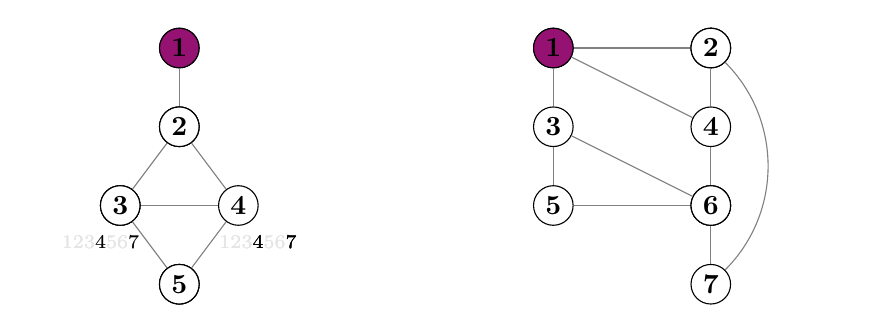
\begin{tikzpicture}%{{{
        \node at (-1, 0) { ~ };
        \node at (9, 0) { ~ };

        \node <1> [draw, circle, fill=white, inner sep=2pt, font=\bfseries] (Na) at (0.75,  0) {1};
        \node <2-> [draw, circle, fill=uofgthistle, inner sep=2pt, font=\bfseries] (Na) at (0.75,  0) {1};

        \node <1-2> [draw, circle, fill=white, inner sep=2pt, font=\bfseries] (Nb) at (0.75, -1) {2};
        \node <3-7> [draw, circle, fill=uofgsunshine, inner sep=2pt, font=\bfseries] (Nb) at (0.75, -1) {2};
        \node <8-> [draw, circle, fill=white, inner sep=2pt, font=\bfseries] (Nb) at (0.75, -1) {2};

        \node <1-5> [draw, circle, fill=white, inner sep=2pt, font=\bfseries] (Nc) at (0, -2) {3};
        \node <6> [draw, forbidden sign, fill=uofgpillarbox, inner sep=2pt, font=\bfseries] (Nc) at (0, -2) {3};
        \node <7-> [draw, circle, fill=white, inner sep=2pt, font=\bfseries] (Nc) at (0, -2) {3};

        \node [draw, circle, fill=white, inner sep=2pt, font=\bfseries] (Nd) at (1.5, -2) {4};

        \node <1-4> [draw, circle, fill=white, inner sep=2pt, font=\bfseries] (Ne) at (0.75, -3) {5};
        \node <5-6> [draw, circle, fill=uofgturquoise, inner sep=2pt, font=\bfseries] (Ne) at (0.75, -3) {5};
        \node <7-> [draw, circle, fill=white, inner sep=2pt, font=\bfseries] (Ne) at (0.75, -3) {5};

        \tikzstyle{edge} = [ultra thick];
        \tikzstyle{ledge} = [color = black!50!white];

        \draw [ledge] (Na) -- (Nb);
        \draw [ledge] (Nb) -- (Nc);
        \draw [ledge] (Nb) -- (Nd);
        \draw [ledge] (Nc) -- (Nd);
        \draw [ledge] (Nc) -- (Ne);
        \draw [ledge] (Nd) -- (Ne);

        \node <1> [draw, circle, fill=white, inner sep=2pt, font=\bfseries] (N1) at (5.5,  0) {1};
        \node <2-> [draw, circle, fill=uofgthistle, inner sep=2pt, font=\bfseries] (N1) at (5.5,  0) {1};

        \node <1-2> [draw, circle, fill=white, inner sep=2pt, font=\bfseries] (N2) at (7.5,  0) {2};
        \node <3-7> [draw, circle, fill=uofgsunshine, inner sep=2pt, font=\bfseries] (N2) at (7.5,  0) {2};
        \node <8-> [draw, circle, fill=white, inner sep=2pt, font=\bfseries] (N2) at (7.5,  0) {2};

        \node [draw, circle, fill=white, inner sep=2pt, font=\bfseries] (N3) at (5.5, -1) {3};

        \node [draw, circle, fill=white, inner sep=2pt, font=\bfseries] (N4) at (7.5, -1) {4};

        \node [draw, circle, fill=white, inner sep=2pt, font=\bfseries] (N5) at (5.5, -2) {5};

        \node <1-4> [draw, circle, fill=white, inner sep=2pt, font=\bfseries] (N6) at (7.5, -2) {6};
        \node <5-6> [draw, circle, fill=uofgturquoise, inner sep=2pt, font=\bfseries] (N6) at (7.5, -2) {6};
        \node <7-> [draw, circle, fill=white, inner sep=2pt, font=\bfseries] (N6) at (7.5, -2) {6};

        \node [draw, circle, fill=white, inner sep=2pt, font=\bfseries] (N7) at (7.5, -3) {7};

        \draw [ledge] (N1) -- (N2);
        \draw [ledge] (N1) -- (N3);
        \draw [ledge] (N1) -- (N4);
        \draw [ledge] (N2) -- (N4);
        \draw [ledge] (N2) to [in=45, out=315] (N7);
        \draw [ledge] (N3) -- (N5);
        \draw [ledge] (N3) -- (N6);
        \draw [ledge] (N4) -- (N6);
        \draw [ledge] (N5) -- (N6);
        \draw [ledge] (N6) -- (N7);

        \node <4-5> [below = 0 of Nc, anchor = north, font=\scriptsize, xshift=-0.25cm] { {\color{black!10!white}{123}}4{\color{black!10!white}{56}}7 };
        \node <4-5> [below = 0 of Nd, anchor = north, font=\scriptsize, xshift=0.25cm] { {\color{black!10!white}{123}}4{\color{black!10!white}{56}}7 };

        \node <6> [below = 0 of Nc, anchor = north, font=\scriptsize, xshift=-0.25cm] { {\color{black!10!white}{1234567}} };
        \node <6> [below = 0 of Nd, anchor = north, font=\scriptsize, xshift=0.25cm] { {\color{black!10!white}{123}}4{\color{black!10!white}{56}}7 };

        \node <7> [below = 0 of Nc, anchor = north, font=\scriptsize, xshift=-0.25cm] { {\color{black!10!white}{123}}4{\color{black!10!white}{56}}7 };
        \node <7> [below = 0 of Nd, anchor = north, font=\scriptsize, xshift=0.25cm] { {\color{black!10!white}{123}}4{\color{black!10!white}{56}}7 };

    \end{tikzpicture}%}}}
\end{frame}

\begin{frame}{Backjumping as a Tree}
    \centering
    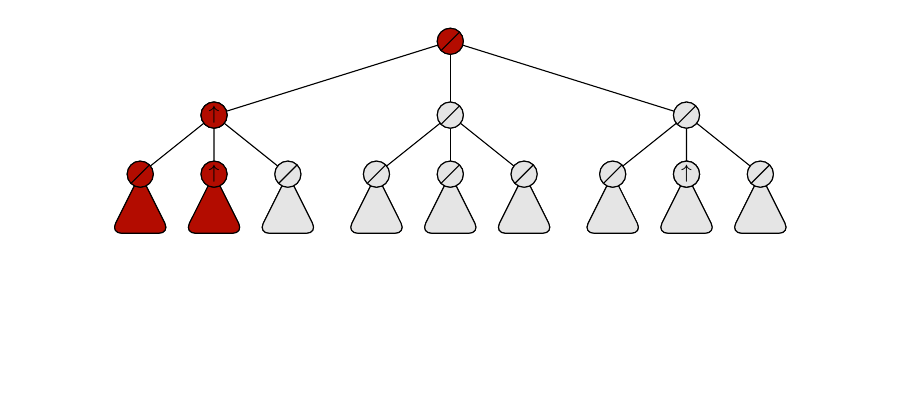
\begin{tikzpicture}[scale=0.75]%{{{
        \coordinate (R);

        \coordinate (N) at (R);

        \coordinate (N1) at ($(N) + (-4, -1.25)$);
        \coordinate (N2) at ($(N) + ( 0, -1.25)$);
        \coordinate (N3) at ($(N) + ( 4, -1.25)$);

        \foreach \na in {1, ..., 3}{
            \coordinate (N\na 1) at ($(N\na) + (-1.25, -1)$);
            \coordinate (N\na 2) at ($(N\na) + ( 0,    -1)$);
            \coordinate (N\na 3) at ($(N\na) + ( 1.25, -1)$);

            \foreach \nb in {1, ..., 3}{
                \coordinate (N\na\nb t1) at ($(N\na\nb) + (-0.5, -1)$);
                \coordinate (N\na\nb t2) at ($(N\na\nb) + ( 0.5, -1)$);

                \coordinate (N\na\nb s1) at ($(N\na\nb) + (-0.3, -0.6)$);
                \coordinate (N\na\nb s2) at ($(N\na\nb) + ( 0.3, -0.6)$);

                \coordinate (N\na\nb h1) at ($(N\na\nb) + (-1.5, -3)$);
                \coordinate (N\na\nb h2) at ($(N\na\nb) + ( 1.5, -3)$);
            }
        }

        \foreach \na in {1, ..., 3}{
            \draw (N) -- (N\na);
            \foreach \nb in {1, ..., 3}{
                \draw (N\na) -- (N\na\nb);
            }
        }

        \tikzstyle{t} = [draw, fill, fill=uofgcobalt, rounded corners];
        \tikzstyle{tf} = [draw, fill, fill=uofgpillarbox, rounded corners];
        \tikzstyle{ts} = [draw, fill, fill=black!10!white, rounded corners];
        \foreach \na in {1, ..., 3}{
            \foreach \nb in {1, ..., 3}{
                \ifthenelse{\na = 1}{
                    \ifthenelse{\na\nb = 11}{
                        \draw <1> [t] (N\na\nb) -- (N\na\nb t1) -- (N\na\nb t2) -- cycle;
                        \draw <2-> [tf] (N\na\nb) -- (N\na\nb t1) -- (N\na\nb t2) -- cycle;
                    }{}
                    \ifthenelse{\na\nb = 12}{
                        \draw <1-2> [t] (N\na\nb) -- (N\na\nb t1) -- (N\na\nb t2) -- cycle;
                        \draw <3-> [tf] (N\na\nb) -- (N\na\nb t1) -- (N\na\nb t2) -- cycle;
                    }{}
                    \ifthenelse{\na\nb = 13}{
                        \draw <1-3> [t] (N\na\nb) -- (N\na\nb t1) -- (N\na\nb t2) -- cycle;
                        \draw <4-> [ts] (N\na\nb) -- (N\na\nb t1) -- (N\na\nb t2) -- cycle;
                    }{}
                }{
                    \draw <1-6> [t] (N\na\nb) -- (N\na\nb t1) -- (N\na\nb t2) -- cycle;
                    \draw <7-> [ts] (N\na\nb) -- (N\na\nb t1) -- (N\na\nb t2) -- cycle;
                }
            }
        }

        \tikzstyle{c} = [draw, circle, fill, fill=uofgcobalt];
        \tikzstyle{cf} = [draw, circle, fill, fill=uofgpillarbox];
        \tikzstyle{cx} = [draw, forbidden sign, fill, fill=uofgpillarbox];
        \tikzstyle{cs} = [draw, forbidden sign, fill, fill=black!10!white];
        \tikzstyle{cfs} = [draw, circle, fill, fill=black!10!white];
        \node <1-7> [c] at (N) { };
        \node <8-> [cx] at (N) { };

        \foreach \na in {1, ..., 3}{
            \ifthenelse{\na = 1}{
                \node <1-4> [c] at (N\na) { };
                \node <5> [cx] at (N\na) { };
                \node <6-> [cf] at (N\na) { };
                \node <6-> [font=\scriptsize] at (N1) { $\uparrow$ };
            }{
                \node <1-6> [c] at (N\na) { };
                \node <7-> [cs] at (N\na) { };
            }

            \foreach \nb in {1, ..., 3}{
                \ifthenelse{\na = 1}{
                    \ifthenelse{\na\nb = 11}{
                        \node <1> [c] at (N\na\nb) { };
                        \node <2-> [cx] at (N\na\nb) { };
                    }{}
                    \ifthenelse{\na\nb = 12}{
                        \node <1-2> [c] at (N\na\nb) { };
                        \node <3-> [cf] at (N\na\nb) { };
                        \node <3-> [font=\scriptsize] at (N12) { $\uparrow$ };
                    }{}
                    \ifthenelse{\na\nb = 13}{
                        \node <1-3> [c] at (N\na\nb) { };
                        \node <4-> [cs] at (N\na\nb) { };
                    }{}
                }{
                    \node <1-6> [c] at (N\na\nb) { };

                    \ifthenelse{\na\nb = 32}{
                        \node <7-8> [cs] at (N\na\nb) { };
                        \node <9-> [cfs] at (N\na\nb) { };
                        \node <9-> [font=\scriptsize] at (N32) { $\uparrow$ };
                    }{
                        \node <7-> [cs] at (N\na\nb) { };
                    }
                }
            }
        }

        \node at (-7, -5.5) { }; \node at (7, -5.5) { };
    \end{tikzpicture}%}}}
    \\~
\end{frame}

\begin{frame}{A Backjumping Algorithm}
    \scriptsize
    
\begin{tikzpicture}[remember picture, overlay]
        \coordinate (fail1lc) at ($(pic cs:fail1l) + (0, 0.13)$);
        \coordinate (fail1rc) at ($(pic cs:fail1r) + (0, 0.03)$);
        \node <3-> (fail1box) [fill=uofgpumpkin, rounded corners, fit=(fail1lc) (fail1rc)] { \phantom{X} };
        \coordinate (fail2lc) at ($(pic cs:fail2l) + (0, 0.13)$);
        \coordinate (fail2rc) at ($(pic cs:fail2r) + (0, 0.03)$);
        \node <3-> (fail2box) [fill=uofgpumpkin, rounded corners, fit=(fail2lc) (fail2rc)] { \phantom{X} };
        \coordinate (fail3lc) at ($(pic cs:fail3l) + (0, 0.13)$);
        \coordinate (fail3rc) at ($(pic cs:fail3r) + (0, 0.03)$);
        \node <3-4> (fail3box) [fill=uofgpumpkin, rounded corners, fit=(fail3lc) (fail3rc)] { \phantom{X} };
        \node <4-> (fail3box) [fill=uofgcobalt, rounded corners, fit=(fail3lc) (fail3rc)] { \phantom{X} };
        \coordinate (fail4lc) at ($(pic cs:fail4l) + (0, 0.13)$);
        \coordinate (fail4rc) at ($(pic cs:fail4r) + (0, 0.03)$);
        \node <3-> (fail4box) [fill=uofgpumpkin, rounded corners, fit=(fail4lc) (fail4rc)] { \phantom{X} };
        \coordinate (fail5lc) at ($(pic cs:fail5l) + (0, 0.13)$);
        \coordinate (fail5rc) at ($(pic cs:fail5r) + (0, 0.03)$);
        \node <3> (fail5box) [fill=uofgpumpkin, rounded corners, fit=(fail5lc) (fail5rc)] { \phantom{X} };
        \node <4-> (fail5box) [fill=uofgcobalt, rounded corners, fit=(fail5lc) (fail5rc)] { \phantom{X} };

        \coordinate (success1lc) at ($(pic cs:success1l) + (0, 0.13)$);
        \coordinate (success1rc) at ($(pic cs:success1r) + (0, 0.03)$);
        \node <2-> [fill=uofglawn, rounded corners, fit=(success1lc) (success1rc)] { \phantom{X} };
        \coordinate (success2lc) at ($(pic cs:success2l) + (0, 0.13)$);
        \coordinate (success2rc) at ($(pic cs:success2r) + (0, 0.03)$);
        \node <2-> [fill=uofglawn, rounded corners, fit=(success2lc) (success2rc)] { \phantom{X} };
        \coordinate (success3lc) at ($(pic cs:success3l) + (0, 0.13)$);
        \coordinate (success3rc) at ($(pic cs:success3r) + (0, 0.03)$);
        \node <2-> [fill=uofglawn, rounded corners, fit=(success3lc) (success3rc)] { \phantom{X} };

        \draw <4-> [->, thick, color=uofgcobalt] (fail3box) -| (fail5box);

        \coordinate (fgets1lc) at ($(pic cs:fgets1l) + (0, 0.13)$);
        \coordinate (fgets1rc) at ($(pic cs:fgets1r) + (0, 0.03)$);
        \node <6-> (fgets1box) [fill=uofgthistle, rounded corners, fit=(fgets1lc) (fgets1rc)] { \phantom{X} };
        \coordinate (fgets2lc) at ($(pic cs:fgets2l) + (0, 0.13)$);
        \coordinate (fgets2rc) at ($(pic cs:fgets2r) + (0, 0.03)$);
        \node <6-> (fgets2box) [fill=uofgthistle, rounded corners, fit=(fgets2lc) (fgets2rc)] { \phantom{X} };
        \coordinate (fgets3lc) at ($(pic cs:fgets3l) + (0, 0.13)$);
        \coordinate (fgets3rc) at ($(pic cs:fgets3r) + (0, 0.03)$);
        \node <6-> (fgets3box) [fill=uofgthistle, rounded corners, fit=(fgets3lc) (fgets3rc)] { \phantom{X} };
        \coordinate (fgets4lc) at ($(pic cs:fgets4l) + (0, 0.13)$);
        \coordinate (fgets4rc) at ($(pic cs:fgets4r) + (0, 0.03)$);
        \node <6-> (fgets4box) [fill=uofgthistle, rounded corners, fit=(fgets4lc) (fgets4rc)] { \phantom{X} };
        \coordinate (fgets5lc) at ($(pic cs:fgets5l) + (0, 0.13)$);
        \coordinate (fgets5rc) at ($(pic cs:fgets5r) + (0, 0.03)$);
        \node <6-> (fgets5box) [fill=uofgthistle, rounded corners, fit=(fgets5lc) (fgets5rc)] { \phantom{X} };
        \coordinate (fgets6lc) at ($(pic cs:fgets6l) + (0, 0.13)$);
        \coordinate (fgets6rc) at ($(pic cs:fgets6r) + (0, 0.03)$);
        \node <6-> (fgets6box) [fill=uofgthistle, rounded corners, fit=(fgets6lc) (fgets6rc)] { \phantom{X} };
    \end{tikzpicture}
    \scriptsize
    \begin{algorithm}[H]
    \DontPrintSemicolon
    \SetKwSwitch{Switch}{Case}{Other}{case}{of}{}{otherwise}{endcase}{endsw}
    \nl $\FuncSty{search}$ (Domains $D$) $\rightarrow$ \tikzmark{fail1l}Fail $F$\tikzmark{fail1r} \KwSty{or} \tikzmark{success3l}Success\tikzmark{success3r} \;
    \nl \Begin{
        \nl \tikzmark{success1l}\lIf {$D = \emptyset$}{$\KwSty{return}~\textnormal{Success}$\tikzmark{success1r}}
        \nl $D_v \gets \textnormal{a domain in $D$ with minimum size}$ \;
        \nl \tikzmark{fgets1l}$F \gets \{ v \}$\tikzmark{fgets1r} \;
        \nl \ForEach {$v' \in D_v~\textnormal{ordered by a heuristic}$}{
            \nl $D' \gets \FuncSty{clone}(D)$ \;
            \nl \Switch{$\FuncSty{assign}(D', v, v')$}{
                \nl \lCase{\textnormal{\tikzmark{fail2l}Fail
                $\tikzmark{fgets5l}F'\tikzmark{fgets5r}$\tikzmark{fail2r}~\KwSty{then}}}{\tikzmark{fgets2l}$F \gets F \cup F'\tikzmark{fgets2r}$}
                \nl \Case{\textnormal{Success~\KwSty{then}}}{
                    \nl \Switch{$\FuncSty{search}(D' - D_v)$}{
                        \nl \Case{\textnormal{\tikzmark{fail3l}Fail $\tikzmark{fgets6l}F'\tikzmark{fgets6r}$\tikzmark{fail3r}~\KwSty{then}}}{
                            \nl \lIf{\only<1-4>{$\nexists\,w \in F'~\KwSty{such that}~D_w \ne
                                D'_w$}\only<5->{\color{black!20!white}$\nexists\,w \in F'~\KwSty{such that}~D_w \ne
                            D'_w$}}{$\KwSty{return}~\tikzmark{fail5l}\textnormal{Fail}~F'\tikzmark{fail5r}$}
                            \nl \tikzmark{fgets3l}$F \gets F \cup F'$\tikzmark{fgets3r} \;
                        }
                        \nl \tikzmark{success2l}\lCase{\textnormal{Success~\KwSty{then}}}{$\KwSty{return}~\textnormal{Success}$\tikzmark{success2r}}
                    }
                }
            }
        }
        \nl $\KwSty{return}~\tikzmark{fail4l}\textnormal{Fail}~\tikzmark{fgets4l}F\tikzmark{fgets4r}\tikzmark{fail4r}$ \;
    }
    \end{algorithm}
\end{frame}

\begin{frame}{Backjumping as a Lazy Fold}
    \begin{itemize}
        \item Lazily map each subproblem to Jump $F$ $\KwSty{or}$ Fail $F$ $\KwSty{or}$ Success.
        \item Lazily fold, starting with Fail $\{ v \}$, as follows:
            \begin{alignat*}{2}
                \underline{\hspace{1em}} &~\circled{$>$}~ \textnormal{Success} \hspace{1em} &&= \textnormal{Success} \\
                \underline{\hspace{1em}} &~\circled{$>$}~ \textnormal{Jump}~F \hspace{1em} &&= \textnormal{Jump}~F \\
                \textnormal{Fail}~F &~\circled{$>$}~ \textnormal{Fail}~G \hspace{1em} &&= \textnormal{Fail}~(F \cup G)
            \end{alignat*}
        \item If a Jump $F$ occurs to the left of a Success, we have a bug.
    \end{itemize}
\end{frame}

\begin{frame}{Folding Zero}
    \begin{itemize}
        \item When multiplying, if any item is 0, the result is 0.
            \begin{alignat*}{2}
                \underline{\hspace{1em}} &~\times~ 0 \hspace{1em} &&= 0 \\
                0 &~\times~ \underline{\hspace{1em}} \hspace{1em} &&= 0
            \end{alignat*}
        \item Here, if any item is Success, the result is Success, and we do not need to evaluate
            the rest of the map.
            \begin{alignat*}{2}
                \underline{\hspace{1em}} &~\circled{$>$}~ \textnormal{Success} \hspace{1em} &&= \textnormal{Success}
            \end{alignat*}
        \item If any item is Jump $F$, the result is either Jump $F$, or some Jump $G$ or Success
            that is further to the left. We do not need to evaluate any item to the right.
            \begin{alignat*}{2}
                \underline{\hspace{1em}} &~\circled{$>$}~ \textnormal{Jump}~F \hspace{1em} &&= \textnormal{Jump}~F
            \end{alignat*}
    \end{itemize}
\end{frame}

\begin{frame}{Preventing a Slowdown, Part 2}
    \begin{itemize}
        \item Any subproblem which we have shown will not be used, must be cancelled (recursively)
            immediately.
        \item When the result of a fold is known, the continuation must be executed immediately.
    \end{itemize}
\end{frame}

\begin{frame}{Some Grumpy Remarks about Brittle Skeletons}
    \only<2>{
        \centering
        \includegraphics*[keepaspectratio=true,scale=0.4]{skeletons1.png}
    }
    \only<3>{
        \centering
        \includegraphics*[keepaspectratio=true,scale=0.4]{skeletons3.png}
    }
    \only<4-5>{
        \centering
        \includegraphics*[keepaspectratio=true,scale=0.4]{skeletons4.png}

        \vspace*{1em}

        \uncover<5>{
            \centering
            \includegraphics* [keepaspectratio=true,scale=0.4]{skeletons5.png}
        }
    }
\end{frame}

\begin{frame}{What's the Alternative?}

    \begin{itemize}
        \item <2-> Doing it by hand?
            \begin{itemize}
                \item This works, but is painful and error-prone\ldots
                \item My current implementation works by keeping a ``sequential'' thread and
                    ``precomputing'' using extra threads. This often leads to the sequential thread
                    being idle and blocking.
                \item Allowing the blocking thread to suspend and steal elsewhere could give an
                    absolute slowdown.
            \end{itemize}

        \item <3-> Better skeletons?
            \begin{itemize}
                \item But they would need to be very domain-specific, which defeats the point of
                    skeletons\ldots
            \end{itemize}

        \item <4-> External descriptions of search?
            \begin{itemize}
                \item I've yet to figure out why this will end up not being very good\ldots
            \end{itemize}
    \end{itemize}

\end{frame}

\begin{frame}[b]
    \begin{center}
    \url{http://dcs.gla.ac.uk/~ciaran} \\
    \href{mailto:c.mccreesh.1@research.gla.ac.uk}{\nolinkurl{c.mccreesh.1@research.gla.ac.uk}}
\end{center}
\begin{tikzpicture}[remember picture, overlay]
    \node at (current page.north west) {\begin{tikzpicture}[remember picture, overlay]\fill
    [fill=uofguniversityblue, anchor=north west] (0, 0) rectangle (\paperwidth, -1.5cm);\end{tikzpicture}};
    \node [anchor=north west, shift={(0.2cm,-0.2cm)}] at (current page.north west) {\includegraphics*[keepaspectratio=true,scale=0.5]{UoG_keyline.pdf}};
\end{tikzpicture}
\end{frame}

\end{document}

